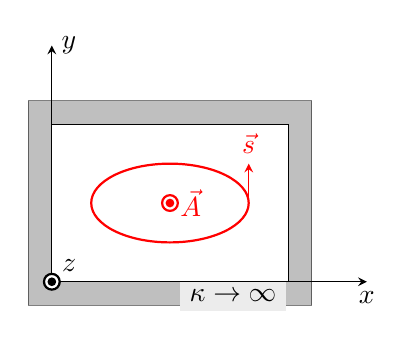
\begin{tikzpicture}
	\draw[fill=gray, opacity=0.5] (-0.3,-0.3) rectangle (3.3,2.3);
	\node[fill=lightgray!30] at (2.3,-0.18){$\kappa\to\infty$};
	\draw[thin, fill=white] (0,0) rectangle (3,2);
	\draw[thin,-stealth] (3,0) -- (4,0) node[below] {$x$};
	\draw[thin,-stealth] (0,2) -- (0,3) node[right] {$y$};
	\draw[fill=white, thick] (0,0) circle (0.1) node[anchor=south west]{$z$};
	\draw[fill=black, thick] (0,0) circle (0.04);
	\draw[red, thick] (1.5,1) circle (1 and 0.5);
	\draw[red, thin,-stealth] (2.5,1) -- +(0,0.5) node[above]{$\dd \vec{s}$};
	\draw[fill=white, thick, draw=red] (1.5,1) circle (0.1) node[anchor=west,color=red]{$\dd \vec{A}$};
	\draw[fill=red, thick, draw=red] (1.5,1) circle (0.04);
\end{tikzpicture}